\documentclass[10pt]{article}
\usepackage{graphicx}
\usepackage{wrapfig}
\author{Justinas Bikulcius, 2095878b}
\title{Distributed Algorithms and Systems 4 (H)\\Assessed Exercise Report}
\date{\today{}}
\begin{document}
\maketitle
\pagebreak

\section{Introduction}
I have developed an auction system using Java 8 and RMI as part of the assessed exercise. My implementation covers all of the requirements that were specified in the exercise document. There is a server that lets the users create auction items, view auctions and make bids. It also notifies bidders when they are outbid or the auction closes, maintains historical records, has the ability save and load its state from file storage. There are two client implementations - one that is to be used by actual users and one that acts as a \textit{Runnable} for multithreaded testing. The clientside also contains a failure detector that can detect and correct connection failures as well as measure performance. The auction system is thread safe to the best of my understanding.

\section{Design}
I have split up this section into three subsections - \textbf{Serverside}, \textbf{Clientside} and \textbf{Testing}. Due to the nature of Java RMI, there are some elements of the system that span all three of these subsections - that is the \textit{IAuctionServer}, \textit{IAuctionClient} and classes that implement these interfaces. However, this section will be written under the assumption that \textit{IAuctionServer} and relevant classes belong to the serverside whilst \textit{IAuctionClient}, naturally, resides in the Clientside.

\subsection{Serverside}
\begin{wrapfigure}[14]{r}{0.5\textwidth}
  \begin{flushright}
    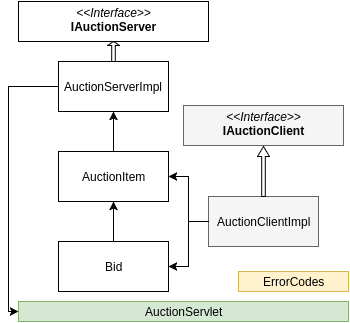
\includegraphics[width=0.48\textwidth]{srv.png}
  \end{flushright}
  \caption{Objects directly related to the server}
\end{wrapfigure}
The auction's serverside contains an \textit{IAuctionServer} interface that extends \textit{Remote}, an enum \textit{ErrorCodes} containing error/success codes and four classes.
\begin{description}
\item [AuctionServerImpl] implements the core functionality of the server.
\item [AuctionItem] represents auction listings, maintains a list of bids and observers for that item and contains some bidding logic.
\item [Bid] a data model with no logic besides the overloaded \textit{toString()} method.
\item [AuctionServlet] runs the whole thing, manages standard IO and loading/saving auction state.
\end{description}
\pagebreak
\subsubsection{Server Implementation}
The majority of the server's logic is distributed between two classes - \textit{AuctionServerImpl} and \textit{AuctionItem}.\par
The \textit{AuctionServerImpl} class serves as the main layer of interaction with the client. It maintains a \textit{ConcurrentHashMap} of open and a \textit{HashMap} of closed auctions. It also has a \textit{Timer} that is used for scheduling tasks that lifecycle (open$\rightarrow$closed$\rightarrow$removed) auction items. All of the methods that create new items or bids have the \textit{IAuctionClient} as the first parameter in order to define object ownership.\par
The \textit{AuctionItem} class has an id, name, owner, minimum bid, closing/opening dates. It also maintains a set of clients (observers) that have bid on the item. This set includes the item owner as well. \textit{AuctionItem} also has methods for making a bid, getting the winning bid and a method for notifying all observers with a message via a callback method.\par 
When a client wants to create an auction item, he invokes the \textit{createAuctionItem()} method. First, a new \textit{AuctionItem} is created. The parameters are validated both inside the function and during item initialisation. Then, the item is put into the open auctions concurrent hashmap. Then, a new \textit{LifecycleAuctionItemTask} is created and scheduled to run when the auction ends. Finally, if there are no errors - a success message is returned.\par
Bidding works in a similar way. After parameter validation, we fetch the \textit{AuctionItem}, create a new \textit{Bid} object and call the \textit{AuctionItem's} method \textit{makeBid()}. This method adds the bid to the \textit{AuctionItem's} bid list, adds the bid's owner to the set of observers and then notifies all observers about the new bid. The method is synchronized because proper concurrent access is important for bidding. Once all of this is done, a success message is returned to the client.\par
There are methods for getting a list of open and closed auctions as a nicely formatted string. The system doesn't return an actual list of AuctionObjects because of two reasons - too much data to transmit and they might contain sensitive data (e.g. other bidders). There is also a void method for probing the system (used by the \textit{FailureDetector}).
\subsubsection{Auction Item Lifecycle}
One of the most important features of the server is being able to lifecycle auction items.\par
Once created, an auction item is put into the concurrent hashmap that holds all open auctions. A new \textit{LifeCycleAuctionItemTask} is created and scheduled using the timer. The task does two things. If the auction is open, it moves it to the hashmap that contains closed auctions, creates a new \textit{LifeCycleAuctionItemTask}, schedules it for the default cleanup period and notifies all observers that the auction has ended. If an auction is already closed - it gets removed permanently. The code in the task's \textit{run()} method runs in a synchronised block.\pagebreak
\subsubsection{Saving and Loading}
The server has the ability to save and load state to file storage. This functionality resides in \textit{AuctionServlet}.\\ \par
Saving  done by simply serializing the \textit{AuctionServerImpl} object and writing it using file IO. Filename can be specified when running the servlet using standard IO. There's also a \textit{TimerTask} for saving the server every 5 minutes. The only problem with this approach is that the \textit{Timer} object in \textit{AuctionServerImpl} can't be serialized. Therefore I'm maintaining a list of timer tasks and every time I load a server state the timer has to be reinitialized and rescheduled.
\subsection{Clientside}
\begin{wrapfigure}[13]{r}{0.5\textwidth}
  \begin{flushright}
    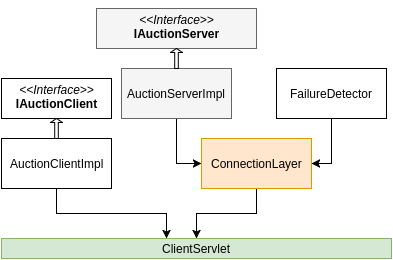
\includegraphics[width=0.48\textwidth]{client.png}
  \end{flushright}
  \caption{Objects directly related to the client}
\end{wrapfigure}
The clientside contains the \textit{IAuctionClient} interface and four classes.
\begin{description}
\item [AuctionClientImpl] a remote class that has a name and a callback.
\item [FailureDetector] responsible for failure detection, correction and performance measurement.
\item [ConnectionLayer] a wrapper that maintains the server object and an instance of the \textit{FailureDetector}
\item [ClientServlet] runs an interactive client
\end{description}
\subsubsection{Client and Connection Layer}
The client is run by launching the \textit{ClientServlet} which instantiates the \textit{AuctionClientImpl} and \textit{ConnectionLayer} objects. The remote class \textit{AuctinClientImpl} is much simpler that the server's remote object. It only holds the name of the client and a callback method that is used by the server. The \textit{ConnectionLayer} contains the \textit{FailureDetector} and the server object. It maintains server connectivity and reinstantiates the server object in case of connection failure. This layer of abstraction is required because when the server object loses connectivity, all subsequent requests fail (even if the server comes back online) so the object has to be reinstantiated. Tracking and managing server connectivity is a slightly messy process, therefore it is better to separate it from code that deals with user interaction.
\subsubsection{Failure Detector}
The failure detector has a \textit{Timer} that runs a \textit{ProbeTask} every 5 (configurable) seconds which simply probes the server. If the server's status is 'disconnected' - we try to fix that by reconnecting. If a \textit{RemoteException} is thrown during probing or reconnection, we assume that the server is dead and set its status to disconnected in the \textit{ConnectionLayer}.\par An another important part of the failure detector is performance measurement. It's done fairly simply - first, we prime the system by running the same probe method that checks the server heartbeat. Then, we capture the current time in milliseconds, run the probe method x times, capture end time and then calculate the average turnaround by dividing the time elapsed by the number of probes.\par The implementation of the failure detector contains more functionality than the auction system is using as I originally intended using sockets to probe the server. There are multiple constructors that can specify timeout or determine it automatically by calculating the turnaround with some specified sensitivity. For example, if the average turnaround is 50ms and the sensitivity is 500ms the server would be assumed dead if there's no response for 550ms.
\subsection{Testing}
Testing is done by running \textit{RunSimulation} which asks the user for the number of worker threads and duration. Then, these worker threads are started and the system gets a performance evaluation by the failure detector every 5 seconds. \textit{AuctionClientWorker} use the following strategy to bid and create items: 
\begin{enumerate}
  \item While the simulation is running, check if there is a specific number of items in the auction (set to the number of threads by default)
  \item If not - create random items until that number is reached
  \item Make bids on random items 
  \begin{itemize}
    \item where the amount is a random number + an ever-increasing counter so bids increase over time
  \end{itemize}
\end{enumerate}
I have tested the system using this tool extensively and have not encountered any issues.
\pagebreak
\section{Performance}
I have tested the performance of the system both on a single machine running 64-bit Linux Mint 18 and on two machines in the lvl6 undergraduate lab in Boyd Orr using \textit{RunSimulation}.\\ \par
The single machine performance depends mostly on random performance fluctuations caused by running the simulation on the same machine. That is evident when observing that as the number of workers increases, the turnaround during the first 5 seconds is huge but then decreases as threads get fully initialised. After that, there is not a lot of difference between 10, 100, 1000 or 2000 auction clients as everything is happening on the same machine. Hence while the mean turnaround increases due to increasing initialisation overhead, the median remains about the same throughout these tests.
\begin{figure}[h]
\begin{center}
\begin{tabular}{ |p{1.2cm}||p{1cm}|p{1cm}|p{1cm}|p{1cm}|p{1cm}|p{1cm}||p{1cm}||p{1cm}|  }
 \hline
 \multicolumn{9}{|c|}{Single machine} \\
 \hline
 Workers & t=5s & t=10s & t=15s & t=20s & t=25s & t=30s & median & mean\\
 \hline
10 & 0.0869 & 0.0499 & 0.0460 & 0.0509 & 0.0499 & 0.0520 & 0.0504 & 0.0559\\
25 & 0.0652 & 0.0451 & 0.0465 & 0.0468 & 0.0456 & 0.0505 & 0.0466 & 0.0499\\
50 & 0.0588 & 0.0646 & 0.1360 & 0.0842 & 0.0645 & 0.0475 & 0.0645 & 0.0759\\
100 & 0.4217 & 0.5270 & 0.5574 & 0.0479 & 0.0464 & 0.0448 & 0.2348 & 0.2742\\
200 & 2.3547 & 0.0514 & 0.0405 & 0.0456 & 0.0448 & 0.0461 & 0.0455 & 0.4305\\
500 & 2.5470 & 0.0592 & 0.0486 & 0.0494 & 0.0469 & 0.0507 & 0.0500 & 0.4669\\
1000 & 2.5252 & 0.0421 & 0.0495 & 0.0443 & 0.0438 & 0.0552 & 0.0469 & 0.4600\\
2000 & 2.0844 & 0.0508 & 0.0434 & 0.0454 & 0.0389 & 0.0451 & 0.0452 & 0.3846\\
 \hline
\end{tabular}
\end{center}
\caption{The results of running the performance test for 30s with different numbers of workers and measuring the turnaround every 5s}
\end{figure}

\pagebreak
Running the simulation with two machines that are in the same network produce similar results to running it on a single machine. It would be interesting to test the system with more machines as running more than a couple of thousands of threads loads the computers and the results get skewed. Performance is unlikely to degenerate at a couple of thousand of local.\par
\begin{figure}[h]
\begin{center}
\begin{tabular}{ |p{1.2cm}||p{1cm}|p{1cm}|p{1cm}|p{1cm}|p{1cm}|p{1cm}||p{1cm}||p{1cm}|  }
 \hline
 \multicolumn{9}{|c|}{Two machines} \\
 \hline
 Workers & t=5s & t=10s & t=15s & t=20s & t=25s & t=30s & median & mean\\
 \hline
10 & 0.2134 & 0.2159 & 0.2149 & 0.2174 & 0.2137 & 0.2184 & 0.215 & 0.2156\\
25 & 0.2060 & 0.2086 & 0.2080 & 0.2057 & 0.2132 & 0.1867 & 0.2070 & 0.2047\\
50 & 0.2020 & 0.1873 & 0.1865 & 0.1817 & 0.2147 & 0.2101 & 0.1946 & 0.1970\\
100 & 0.1830 & 0.1774 & 0.1738 & 0.1752 & 0.2144 & 0.2135 & 0.1802 & 0.1895\\
200 & 0.1779 & 0.1750 & 0.1818 & 0.1839 & 0.2127 & 0.2081 & 0.1828 & 0.1899\\
500 & 0.6456 & 1.0070 & 0.2162 & 0.2159 & 0.2104 & 0.2159 & 0.2160 & 0.4185\\
1000 & 2.5008 & 0.2107 & 0.2226 & 0.2228 & 0.2121 & 0.2117 & 0.2173 & 0.5967\\
2000 & 2.6497 & 0.2125 & 0.2068 & 0.2004 & 0.2098 & 0.2063 & 0.2083 & 0.6145\\
 \hline
\end{tabular}
\end{center}
\caption{One machine acts as a server, the other runs \textit{RunSimulation}. Again - 30s, multiple workers, turnaround every 5s}
\end{figure}

\begin{figure}[h]
\begin{center}
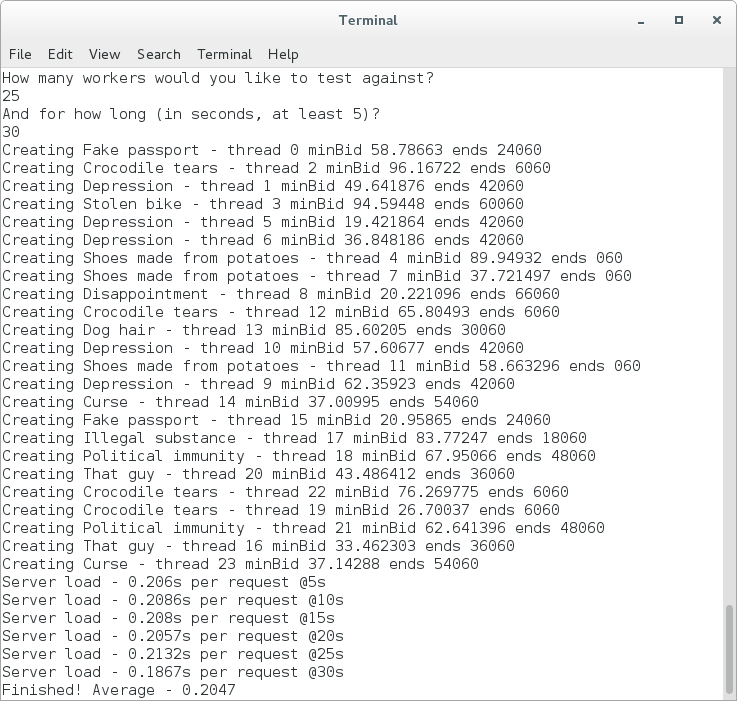
\includegraphics[scale=0.25]{25-30.png}
\caption{Simulation runner (stdio was disabled during actual tests)}
\end{center}
\end{figure}

\pagebreak
\section{Potential extensions}
There are numerous ways to improve the server.
\begin{enumerate}
\item An additional serverside layer for serving requests using a queue could give more insight to server load. The number of clients that are currently connected would be beneficial as well but would require a more elaborate module for gathering statistics over time in order to be useful.
\item There should be a proper authentication system that accepts the username/password combination so users can login after disconnecting. Right now the list of auction participants (observers) contains client objects and if they get reinstantiated - the server will fail to notify them.
\item Item listings should have paging as it is not wise to send the whole list of items over the network in case there's thousands of items. Displaying them can be a challenge as well.
\item Serializing the server object might not be the best way to save server state to persistent storage. The \textit{Timer} object is not serializable so my implementation maintains a list of \textit{TimerTasks} so they can get rescheduled after loading a state. There would be a great saving of memory if we were to use some kind of a database, e.g. SQLite.
\item My implementation holds open auctions in a concurrent data structure. It would be better to manage concurrency manually as there are some drawbacks to this approach. I use synchronized blocks and methods only when it is absolutely necessary so there's less blocking but the concurrent hashmap is most likely the bottleneck.
\item Reorganisation of \textit{ConnectionLayer} - the failure detector should be optional and set using some method rather than passing failure detector parameters in the \textit{ConnectionLayer} constructor. Server methods could be moved to \textit{ConnectionLayer} because calling \textit{connectionLayer.getServer()} every time seems suboptimal.
\item Sockets usage for failure detection and performance measurement would provide more control and better readings. There should also be an option to set max retries when reconnecting.
\item Data model extensions - additional fields for \textit{Bid} and \textit{AuctionItem}, e.g. description or condition.
\end{enumerate}
\pagebreak
\section{How to Run and Test the System}
\begin{figure}[h]
\begin{center}

\includegraphics[scale=0.6]{runopt.png}
\caption{Three shell scripts that run different parts of the system}
\end{center}
\end{figure}
The easiest way to run the system is by running the shell scripts that are in the root directory. These can be executed using the terminal, by running ./runx.sh. Alternatively, the system can be compiled using 
\begin{verbatim}
find ./src -name "*.java" | xargs javac
\end{verbatim}
and run with 
\begin{verbatim}
java -cp ./src client.ClientServlet
java -cp ./src server.AuctionServlet
java -cp ./src test.RunSimulation
\end{verbatim}
\par
Usage of these three interactive applications is self explanatory - just select the appropriate option and press enter. If there's a need to change the host or port - add them as commandline parameters, e.g.
\begin{verbatim}
java -cp ./src server.AuctionServlet "127.0.0.1" 8080
\end{verbatim}
\par
I do not provide a saved server state with prepopulated content because I am not sure when the system would be tested (the auctions might expire by then). If there is a need to populate the server with some random items and bids - run the server and then run the simulation with a couple of workers. This will populate the server with some random data and then the client can be used to observe the auction.
\par
Performance testing can be done either by using the client (there's an option to check server load) or running the simulation.\\ \\
\textbf{Important note:} For testing to be more accurate, turn off logging by changing line 82 in file \textit{/home/justas/Uni/DAS/2095878b/src/server}
\begin{verbatim}
LOGGER.setLevel(Level.ALL);
\end{verbatim}
to
\begin{verbatim}
LOGGER.setLevel(Level.OFF);
\end{verbatim}
as standard IO hogs resources.
\end{document}
